%-------------------------
% Resume in Latex
% Author : Jake Gutierrez
% Based off of: https://github.com/sb2nov/resume
% License : MIT
%------------------------

\documentclass[letterpaper,11pt]{article}

\usepackage{latexsym}
\usepackage[empty]{fullpage}
\usepackage{titlesec}
\usepackage{marvosym}
\usepackage[usenames,dvipsnames]{color}
\usepackage{verbatim}
\usepackage{enumitem}
\usepackage[hidelinks]{hyperref}
\usepackage{fancyhdr}
\usepackage[english]{babel}
\usepackage{tabularx}
\usepackage{fontawesome5}
\usepackage{multicol}
\usepackage{wasysym}
\usepackage{lastpage}


\usepackage{tikz}
\usepackage{graphicx}

\setlength{\multicolsep}{-3.0pt}
\setlength{\columnsep}{-1pt}
\input{glyphtounicode}
\usepackage{fontawesome5}

\newcommand{\portfoliosymbol}{\faFolderOpen\hspace{-.1em}\faBriefcase}

\pagenumbering{arabic}
\usepackage{xcolor} % to use colors
\definecolor{Blue}{HTML}{0000FF}


%----------FONT OPTIONS----------
% sans-serif
% \usepackage[sfdefault]{FiraSans}
% \usepackage[sfdefault]{roboto}
% \usepackage[sfdefault]{noto-sans}
% \usepackage[default]{sourcesanspro}

% serif
% \usepackage{CormorantGaramond}
% \usepackage{charter}


\pagestyle{fancy}
\fancyhf{} % clear all header and footer fields
\fancyfoot{}
\renewcommand{\headrulewidth}{0pt}
\renewcommand{\footrulewidth}{0pt}

% Adjust margins
\addtolength{\oddsidemargin}{-0.6in}
\addtolength{\evensidemargin}{-0.5in}
\addtolength{\textwidth}{1.19in}
\addtolength{\topmargin}{-.7in}
\addtolength{\textheight}{1.4in}

\urlstyle{same}

\raggedbottom
\raggedright
\setlength{\tabcolsep}{0in}

% Sections formatting
\titleformat{\section}{
  \vspace{-4pt}\scshape\raggedright\large\bfseries
}{}{0em}{}[\color{black}\titlerule \vspace{-5pt}]

% Ensure that generate pdf is machine readable/ATS parsable
\pdfgentounicode=1

%-------------------------
% Custom commands
\newcommand{\resumeItem}[1]{
  \item\small{
    {#1 \vspace{-2pt}}
  }
}

\newcommand{\classesList}[4]{
    \item\small{
        {#1 #2 #3 #4 \vspace{-2pt}}
  }
}

\newcommand{\resumeSubheading}[4]{
  \vspace{-2pt}\item
    \begin{tabular*}{1.0\textwidth}[t]{l@{\extracolsep{\fill}}r}
      \textbf{#1} & \textbf{\small #2} \\
      \textit{\small#3} & \textit{\small #4} \\
    \end{tabular*}\vspace{-7pt}
}

\newcommand{\resumeSubSubheading}[2]{
    \item
    \begin{tabular*}{0.97\textwidth}{l@{\extracolsep{\fill}}r}
      \textit{\small#1} & \textit{\small #2} \\
    \end{tabular*}\vspace{-7pt}
}

\newcommand{\resumeProjectHeading}[2]{
    \item
    \begin{tabular*}{1.001\textwidth}{l@{\extracolsep{\fill}}r}
      \small#1 & \textbf{\small #2}\\
    \end{tabular*}\vspace{-7pt}
}

\newcommand{\resumeSubItem}[1]{\resumeItem{#1}\vspace{-4pt}}

\renewcommand\labelitemi{$\vcenter{\hbox{\tiny$\bullet$}}$}
\renewcommand\labelitemii{$\vcenter{\hbox{\tiny$\bullet$}}$}

\newcommand{\resumeSubHeadingListStart}{\begin{itemize}[leftmargin=0.0in, label={}]}
\newcommand{\resumeSubHeadingListEnd}{\end{itemize}}
\newcommand{\resumeItemListStart}{\begin{itemize}}
\newcommand{\resumeItemListEnd}{\end{itemize}\vspace{-5pt}}

%-------------------------------------------
%%%%%%  RESUME STARTS HERE  %%%%%%%%%%%%%%%%%%%%%%%%%%%%


\begin{document}

%----------HEADING----------
% \begin{tabular*}{\textwidth}{l@{\extracolsep{\fill}}r}
%   \textbf{\href{http://sourabhbajaj.com/}{\Large Sourabh Bajaj}} & Email : \href{mailto:sourabh@sourabhbajaj.com}{sourabh@sourabhbajaj.com}\\
%   \href{http://sourabhbajaj.com/}{http://www.sourabhbajaj.com} & Mobile : +1-123-456-7890 \\
% \end{tabular*}
\parbox{3.0cm}{%

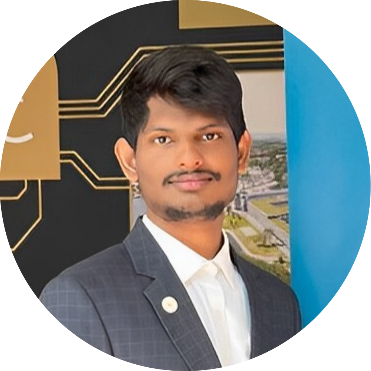
\includegraphics[width=2.7cm,clip]{images/resume_pic_m.png}}
}
\parbox{\dimexpr\linewidth-3.8cm\relax}{
\vspace{-20pt}
\begin{tabularx}{\linewidth}{L r} \\
    {\Huge \scshape  Venkata Sai Yakkshit Reddy Asodi}~
    \href{https://www.cedzlabs.com/yakkshit}{\vspace{1pt}}\\
      Karlskrona, Sweden. \\ \vspace{1pt}
     \small \raisebox{-0.1\height}\faPhone\ +46 0793550685 ~ \href{mailto:saiyakkshit2001@gmail.com}{\raisebox{-0.2\height}\faEnvelope\  {saiyakkshit2001@gmail.com}} ~ 
    \href{https://linkedin.com/in/yakkshit/}{\raisebox{-0.2\height}\faLinkedin\ {yakkshit}}  ~
    \href{https://yakkshit.com/}{\raisebox{-0.2\height}\faGlobe\ {yakkshit.com}}  ~
    \href{https://github.com/yakkshit}{\raisebox{-0.2\height}\faGithub{ saiyakkshit}}
    \vspace{-8pt}
    
\end{tabularx}
}




\vspace{-10pt}

%-----------------------------------

\href{https://www.yakkshit.com/#details}{\section{\textcolor{Black}{Summary} \faLink}
I am a \textbf{Software Developer} with a passion for building high-quality software. I have experience in \textbf{Application development} and have contributed to the product lifecycle, from requirements analysis to deployment. I have a strong understanding of authentication and authorization, and I effectively manage monitoring and logs using tools such as Prometheus, 
Jenkins, 
Grafana, 
GCP CLI. 
I have hands-on experience with \textbf{CI/CD, DevOps, infrastructure as code, and GitHub Version Control}. I have extensive experience in implementing professional practices such as Agile methodologies and Experienced in Java and python.}






 %-----------EDUCATION-----------

%-----------EXPERIENCE-----------
\section{\href{https://www.linkedin.com/in/yakkshit/}{Experience  \faLink}}
  \resumeSubHeadingListStart
  \resumeSubheading
      {BetaTesting.Inc}{Jan 2023 -- June 2023}
      {Application Tester}{\faMapMarker Remote}\\
      \vspace{10pt}
      % \textbf{Description:}
      % I Have worked as a beta tester for the Web Application, identifying and reporting bugs to the development team, and developed problem-solving skills and attention to detail through this experience. I have also learned to work collaboratively with a team to improve user experience and web security.\\
      \textbf{Responsibilities:}
      \resumeItemListStart
      \vspace{-10pt}
        \resumeItem{Conducted beta testing for new Application by developing a comprehensive test plan, executing test cases, and identifying/reporting 25+ critical bugs to the development team; reduced the overall bug rate by 40\%.}
        \resumeItem{The following testing methods Functional, Load, Security, Compatibility, Usability, Automated Testing to enhance the performance of the Application.}
        \resumeItem{Utilizing Tracing method as the development environment to visualize and analyze the application and Leveraging performance analysis.}
    \resumeItemListEnd
    \vspace{-3pt}
    \textbf{Environment:}\emph{Bug reporting, debugging, problem-solving, collaboration, Selenium.}
    \vspace{-5pt}

    \resumeSubheading
      {cedzlabs.com}{May 2021 -- Dec 2022}
      {FullStack Engineer}{\faMapMarker Remote}\\
      \vspace{10pt}
      % \textbf{Description : }As a Full-Stack Engineer at CedzLabs, I was responsible for creating and maintaining both the front-end and back-end components of websites and web applications. I worked with a range of programming languages and technologies, including HTML, CSS, JavaScript, Node.js, Django, and SQL databases.\\
\textbf{Responsibilities : }
      \vspace{-5pt}
      \resumeItemListStart
        \resumeItem{Utilized a range of programming languages and technologies to create and maintain websites and web applications.}
        \resumeItem{Implemented the Django framework to enhance the functionality and interactivity of websites.}
        \resumeItem{Integrated various RESTful APIs to enhance the functionality and features of websites.}
        \resumeItem{Monitored website performance using Google Search Console, Google Analytics, and Firebase Performance SDK.}\\

      \resumeItemListEnd
\vspace{0.5pt}
\textbf{Environment:}\emph{HTML, CSS, JavaScript, Node.js, SQL databases, Django, Google Search Console, Google Analytics, Firebase Performance SDK.}
  
    \resumeSubheading
      {VERZEO.INC}{Aug 2020 -- Mar 2021}
      {AI Engineer Intern}{ \faMapMarker Remote}\\
      \vspace{10pt}
      % \textbf{Description : }I developed a Python project that uses computer vision and deep learning to detect face masks and human falls. The project achieved 95\%\ accuracy for face mask detection and 85\%\ accuracy for human fall detection. It can be used in a variety of applications, such as monitoring compliance with COVID-19 safety regulations. This project is a valuable contribution to the field of computer vision.\\

\textbf{Responsibilities : }
      \vspace{-5pt}
      \resumeItemListStart
        \resumeItem{Utilized Python, TensorFlow, OpenCV, and deep learning techniques to implement the project, working with a provided dataset.}
        \resumeItem{Integrated the trained model into a real-time face mask detection system using the OpenCV library and its computer vision capabilities.}
        \resumeItem{Conducted comprehensive testing to ensure the precision and reliability of the face mask detection system.}
        \\
      \resumeItemListEnd
\vspace{-3pt}
\textbf{Environment:}\emph{Python, TensorFlow, OpenCV, Keras, Deep learning.}
\resumeSubHeadingListEnd

%-----------PROJECTS-----------
\section{\href{https://www.yakkshit.com/#project-1}{Projects } }
    \resumeSubHeadingListStart
    
%---------------------------------------------------------------------------
                
                            % Bachlore Thesis
% -----------------------------------------------------------------------------

 \resumeProjectHeading
          {\textbf{\href{https://www.yakkshit.com/#project-1}{Analysis of Webxr and Arcore}} $|$ \emph{Bachelor Thesis \faGithub}}{June 2023}\\
          \vspace{9pt}
          \vspace{-8pt}
          \resumeItemListStart
            \resumeItem{An augmented reality (AR) application for Android and web was developed using Firebase as a backend-as-a-service (BaaS) platform.}
            \resumeItem{The Android application was created using the ARCore API in Android Studio in the Kotlin programming language.}
            \resumeItem{The web application was built using the Three.js engine and web development frameworks.}
            \resumeItem{The GUI and hardware tests were conducted using system tracing methods, and the test results are being analyzed using machine learning algorithms such as KNN, Random Forest.}
            \resumeItem{Demonstrated proficiency in using system tracing tools to analyze and optimize performance. Experience with the TensorFlow Profiler, as well as library-specific profiling tools. Familiarity with general-purpose system tracing tools, such as strace and perf, which allow for tracing system calls and analyzing system performance at a low level.}
          \resumeItemListEnd 
          \textbf{Tools:}\emph{
                                Kotlin / Java, Threejs , Webxr, , Machine Learning, Gui, hardware Testing, Data analysis.}


%---------------------------------------------------------------------------
                
                            % 2048 Game
% -----------------------------------------------------------------------------

 \resumeProjectHeading
          {\textbf{\href{https://github.com/yakkshit/2048-3d-master.git}{2048 3d game}} $|$ \emph{CI/CD, Unity \faGithub}}{February 2023}\\
          \vspace{9pt}
          \vspace{-8pt}
          \resumeItemListStart
            \resumeItem{I have used Unity Engine for the development of the 2048 3D game.}
            \resumeItem{The script was return in c\#\ .}
            \resumeItem{The Asserts being imported from Unity store.}
            \resumeItem{The game is being deployed in both Web and Android.}
          \resumeItemListEnd 
          \textbf{Tools:}\emph{
                                Unity Engine, C\#\ , WebGL, android, continuous integration.}
         


%---------------------------------------------------------------------------
                
                            % Langversation
                            
% -----------------------------------------------------------------------------

    \resumeProjectHeading          {\textbf{\href{https://github.com/saiyakkshit/Langversation}{Langversation}} $|$ \emph{CI/CD, Android Studio \faGithub}}{December 2022}\\
          \vspace{6pt}
          \textbf{Description:}
         
          \vspace{-8pt}
          \resumeItemListStart
            \resumeItem{ Langversation is a communication, end‑to‑end encrypted multilingual chat‑based android application which was developed in kotlin.}
            \resumeItem{In the development of user conversation i have used XML as front end and Kotlin for the back end.}
            \resumeItem{For the storage and authentication which was used in the app was done in FirebaseStorage and FirebaseAuthentication.}
            \resumeItem{Ml kit translational API which was used to convert from one language to the other.}
            \resumeItem{The Performance and Crashes of the App was monitered using the Firebase Performance SDK and Firebase Crashlytics SDK.}
          \resumeItemListEnd 
          \textbf{Tools:}\emph{
Kotlin, java, ML kit, Firebase, XML.}

%---------------------------------------------------------------------------
                
                            % End
% -----------------------------------------------------------------------------


%-----------EDUCATION-----------
\section{Education Details  \faGraduationCap   }

% \hfill \textbf{\LARGE 
%  \raisebox{9pt} {Software Developer}}
 
  \resumeSubHeadingListStart
    \resumeSubheading
      {Blekinge Institute of Technology}{Sep. 2022 -- June. 2023}
      {Bachelor of Science in Computer Science}{\faMapMarker  Karlskrona, Sweden.}
  \resumeSubHeadingListEnd
    \vspace{-7pt}
  \resumeSubHeadingListStart
    \resumeSubheading
      {University College Of Engineering Jntuk}{Aug. 2019 -- Jun. 2022}
      {Bachelor of Science in Computer Science}{\faMapMarker  AndhraPradesh, India.}
  \resumeSubHeadingListEnd
  \vspace{-10pt}

%-----------PROGRAMMING SKILLS-----------
\section{\href{https://www.linkedin.com/in/yakkshit/details/skills/}{Technical Skills} \faLink}
 \begin{itemize}[leftmargin=0.15in, label={}]
    \small{\item{
     \textbf{Deployment/Automation/templating tools : }{Jenkins, Docker, Github, Bitbucket/Gitlab.} \\
     \textbf{Frameworks : }{Django, TensorFlow, flutter.}\\
     \textbf{Languages : }{ Python, Java/Kotlin, Dart, C, HTML, CSS, JS, php, SQL, TypeScript.}\\
    }}
 \end{itemize}
 \vspace{-17pt}

 
%------RELEVANT COURSEWORK-------
\section{\href{https://www.linkedin.com/in/yakkshit/details/courses/}{Relevant Coursework} \faLink}
    %\resumeSubHeadingListStart
        \begin{multicols}{4}
            \begin{itemize}[itemsep=-4pt, parsep=3pt]
                \item\small Data Structures
                \item Software Methodology
                \item Algorithms Analysis
                \item Database Management
                \item Network Slicing
                \item Information Technology
                \item RESTful API
                \item Computer Architecture \\
                \item UI/UX
                \item IOT
                \item microservices
                \item System Administration\\
            \end{itemize}
        \end{multicols}
        \vspace*{2.0\multicolsep}
    %\resumeSubHeadingListEnd
%-----------INVOLVEMENT---------------
\section{\href{https://www.linkedin.com/in/yakkshit/details/certifications/}{Certificates / Achivements} \faLink}
            \resumeItemListStart
            \resumeItem{\href{https://portal.certiport.com/Portal/Pages/PrintTranscriptInfo.aspx?action=Cert&id=395&cvid=ej8fNHXiWfEntRn/kBIQHw==}{I have Achieved
                MTA(Microsoft Technical Associate)-Python}}
                \vspace{-2pt}
                \resumeItem{\href{https://drive.google.com/file/d/1dhl67D-8GIbrHul7yOXaZnMi9Wy8rkg4/view}{I have Completed as a AI - Intern at Verzeo.inc}}
                \vspace{-2pt}
                \resumeItem{\href{https://portal.certiport.com/Portal/Pages/PrintTranscriptInfo.aspx?action=Cert&id=398&cvid=QiBkzVlVnojF0hDdRTf01Q==}{I have Achieved
                MTA(Microsoft Technical Associate)-Java}}
                \vspace{-2pt}
                \resumeItem{\href{https://www.cloudskillsboost.google/public_profiles/6bf05c97-e7a5-48b7-bd37-03938dae9743}{I have Achieved a Skill badges at Google Cloud carrier path}}
                \vspace{-2pt}
                \resumeItem{\href{https://www.linkedin.com/in/yakkshit/details/certifications/}{I have Achieved azure Certificates and many other Related to Software Development.}}
                
                
            \resumeItemListEnd

            \vspace{-5pt}

%-----------INVOLVEMENT---------------
\section{Leadership / Extracurricular / Contributions}
            \resumeItemListStart
                \vspace{-3pt}\resumeItem{\href{https://cedzlabs.com}{Led a chapter of 30+ members to work towards goals that improve and promote CedzLabs community service, with collaborative environment, academics, and unity.}}\\
                \resumeItem{I contributed to Kubernetes is Developed new functions in the release script to ensure a smooth and error-free release process by checking dependencies, generating release notes for microserves and uploading the final tarball to a remote storage location.}
                % \vspace{-7pt}
                \resumeItem{\href{https://github.com/yakkshit/charm-microk8s/pull/2/files}{I have contributed to adding a new class, MicroK8sClusterUpgradeEvent, to the Micro K8 Cluster and implemented upgrade logic to handle it for performing necessary upgrade logic for the Micro K8s cluster.}}
                \resumeItem{I have extensive experience in implementing professional practices such as Agile methodologies including Scrum and Kanban.}
                
                
            \resumeItemListEnd
    \textbf{Strengths : }\emph{Leadersip skills,
Multitasking, decision making,
Attention to details.
}
\end{document}

